\documentclass[tikz,border=0pt]{standalone}

\usepackage{graphicx}
\usepackage{amsmath, amssymb}
\usetikzlibrary{arrows.meta}


\newcommand{\C}{\mathbb{C}}
\newcommand{\CP}{\C P}

\begin{document}

\begin{tikzpicture}
    \node[anchor=south west, inner sep=0] at (0,0) {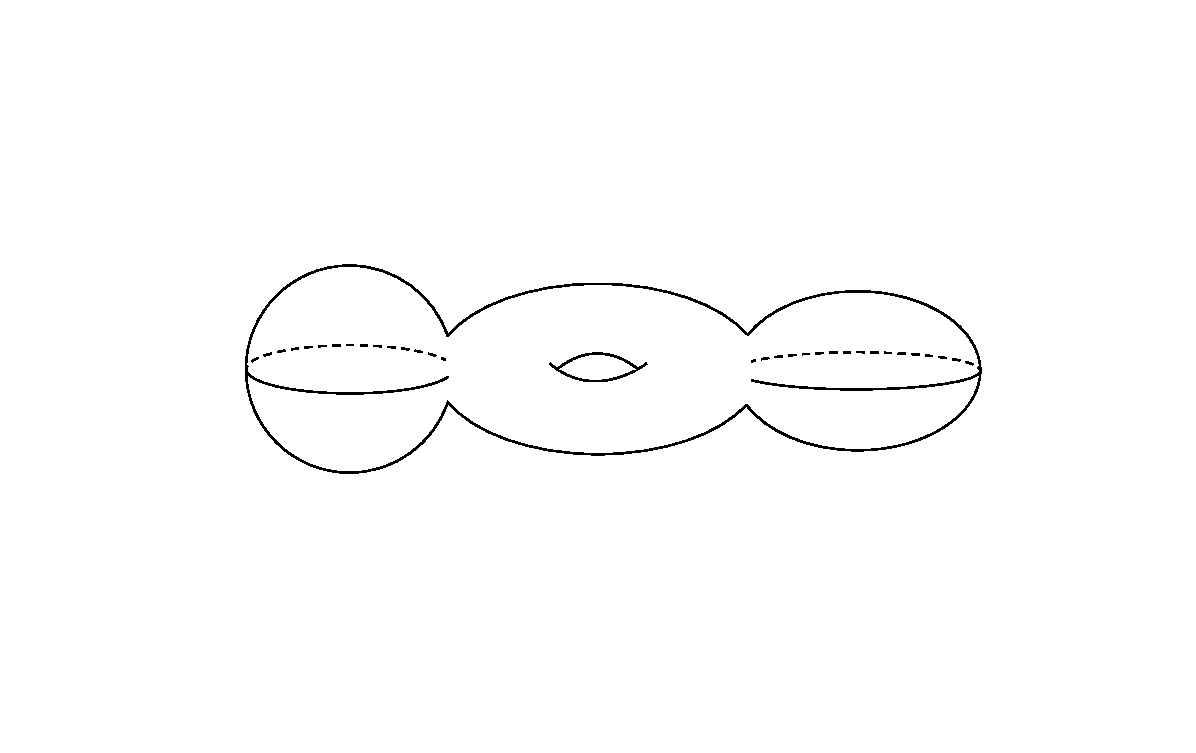
\includegraphics[trim = 4cm 4.5cm 3.5cm 4cm, clip]{main_construction_raw.pdf}};

    \node at (2,-0.5) {\large $\CP^n$};
    \node at (4.15,-0.5) {\large \#};
    \node at (6.3,-0.5) {\large $T^{2n}$};
    \node at (8.45,-0.5) {\large \#};
    \node at (10.6,-0.5) {\large $N$};

    \node at (2,5.5) {\large $S^{2n+1}$};
    \node[anchor=center] at (6.1,5.5) {\large trivial};
    \node[anchor=center] at (10.6,5.5) {\large trivial};

    \node (M) at (-1.5,-0.5) {\large $M$};
    \node at (-0.5,-0.55) {\large $=$};
    \node (E) at (-1.5,5.5) {\large $E$};
    \node at (-0.5,5.45) {\large $=$};

    \draw[-{Stealth}, thick, shorten <= .5cm, shorten >= .5cm] (E) -- (M);


\end{tikzpicture}

\end{document}

